\documentclass[12pt, parskip=full*, abstract]{scrartcl}
\usepackage{stil}

\addbibresource{bibliography.bib}

% \title{Consequences of the sun}
\title{Titan's interaction with Saturn's magnetosphere}

\author{Alexander Ek, John Persson, Björn Sundin}

\begin{document}
\maketitle
\vspace{5mm}
\begin{abstract}
	In this brief non-systematic literature review we attempt to summarize the scientific knowledge about Titan's interaction with the Kronian magnetosphere.
\end{abstract}

\tableofcontents
\newpage

\section{Introduction}
\subsection{Missions to Saturn}

% Cassini-Huygens was launched in 
% Pioneer 11, Voyager 2, Voyager 1, Cassini-Huygens
\subsection{Saturn's magnetosphere}
% Describe the different regions of the magnetosphere
% Sources and sinks of plasma

\subsection{About Titan}
Titan was discovered in 1655 by Christiaan Huygens, it is Saturn's largest moon and the second largest moon in the solar system \parencite{fundamental-planetary-science}. It is an icy moon with a radius of \SI{2575}{\kilo\metre}, a density of \SI{1880}{\kilogram\per\metre^3} and a surface pressure of 1.44 bar. Unlike most moons, Titan has a very dense atmosphere, being even thicker than Earth's and consisting mainly of nitrogen and a smaller amount of methane. Titan has no intrinsic magnetic field but having an orbit at 20 Saturn radii places it near the boundary of the varying Saturnian magnetic field. This combination of a dense atmosphere and the lack of an intrinsic megnetic field and its interaction with the surrounding plasma is therefore unlike that of any other moon in the solar system. 


\section{Interactions between Titan and Saturn's magnetosphere}





















\subsection{Titan's plasma environment}
A 2009 study by \textcite{Rymer-class} classifies Titan's plasm environment into four different categories based on electron thermal data from 54 encounters on titan by Cassini as follows. 

\subsubsection{plasma sheet}
The plasmasheet contains high energy electrons whose peak enegy is on the oder of 100s eV. The electron density is also high in this region with fluxes at $10^6cm^{-2}s^{-1}sr^{-1}$. This was the most common environment, with 19 encounters. \parencite{Rymer-class}

\subsubsection{Lobe-like}
This class also has high energy electrons, with peak energies similar to or higher than that of the plasmas sheet. The electron density is however smaller with fluxes an order of magnitude less. 8 encounters with this environment was made.\parencite{Rymer-class}

\subsubsection{Magnetosheath}

This region is encountered outside of the magnetopause, and thus consists of plasma from the solar wind. In this region electrons are of lower energy, but higher density than the previous two classes. 2 encounters with this environment was made.\parencite{Rymer-class}

\subsubsection{Bi-modal}
This classification is highly variable, containg two seperate electron populations, hence bi-modal. One is similar in energy to the plasma sheet or Lobe-like category. The other population is less energetic but more dense and consists of so called local pick-up population that comes from a neutral cloud, where produced electrons are quickly picked up by the co-rotation with Saturn gaining energy in the order of tenths of eV. The electron energy seen is higher though, which is thought to be explained by these electrons originating from photoionization of larger ions where the energy released is on the order of 10eV. These heavy ions are believed to be water groups, which originate in the inner magnetosphere of Saturn, from the moon Enceladus and migrates outwards to Titan. 5 encounters of this environment was made.\parencite{Rymer-class}

\subsubsection{Implications on Kronian magnetopause}
A 2014 paper by \textcite{Smith-WithOrWithoutTitan} further examines more encounters by cassini, establishing that 45\% of encounters are plasma sheath, 38\% are lobe-like, 6\% magnetosheath. The plasma envionment along Titans obit, when the planet is not cuently precent is also examined, here 55\% of encountes are plasma sheath, 24\% are lobe like and 12\% are magnetosheath. This suggest that the precence of Titan lowers the probablity of expeiencing the magnetosheath, meaning that Titan extends the magnetopause of Saturn outwards.
The authors cannot conclude this however, due to possible sampling bias that needs to be analysed more rigouresly \parencite{Smith-WithOrWithoutTitan}. An earlier paper by \textcite{Wei-WithOrWithoutTitan} draws a similar conclution. This study looks at the specific time intervall of 0900 - 1500 Saturn local time (SLT) and examines the plasma environment in 26 cases with Titan precent and 37 without. The percentage of time in the magnetosheath was 3.37\% near Titan 10.37\% away from Titan, which is statistically significant. The implication of this is that the compressation of the plasma is hindered by Titans' precence \parencite{Wei-WithOrWithoutTitan}.  

\subsubsection{Implications on ionization}
\textcite{Smith-WithOrWithoutTitan} also finds that the bi-modal environment is more prevelant in the vicinity of Titan compared to the orbit of Titan without the moon precent. This suggests that ionization is greater with Titan precent, as the origin of the low energy population of the bi-modal environment is thought to be pick up ions \parencite{Smith-WithOrWithoutTitan}. 

\subsubsection{Additional classification}%Maybe unneccessary //John
An additional classification of the plasma environment, dubbed dense plasma region is also recognized. In this environment the electron energies can be compared to the low energy plasma of the Bi-modal environment, but the higher energy electrons seen in the Bi-modal environment are not precent. Additionally, the environment is more long lived than the Bi-modal low energy electrons. This environment was seen during dusk, no theory of its origin could be found \parencite{Smith-WithOrWithoutTitan}.





































\subsection{Titan's induced magnetosphere}

There are two flows of charged particles across Titan; one is from the Sun and one is from Saturn's magnetospheric plasma \parencite{ionosphere-magnetosphere-interaction-coates}. Due to friction in Saturn's atmosphere and ionosphere, the plasma rotates with the same period as Saturn spins about its axis \parencite{solar-system-magnetospheres}, which is approximately \SI{10.5}{\hour} \parencite{fundamental-planetary-science}. Meanwhile, Titan's rotation period around Saturn is 15.9 days. Neglecting the eccentricity of Titan ($e\approx0.03$) and noting that Titan orbits with a semimajor axis of $a=\SI{1222}{\mega\metre}$, this implies that the magnetospheric plasma flows at a velocity of approximately
\begin{equation}
	2\pi a\left(\frac{1}{T_\text{plasma}} - \frac{1}{T_\text{titan}}\right)\approx\SI{198}{\kilo\metre\per\second}
\end{equation}
relative to Titan. The ram side of this plasma flux is therefore \say{behind} Titan rather than in front. The flow of particles from the sun and from the magnetospheric plasma have two different directions which change during the local day on Titan, see Figure \ref{wakes} \parencite{ionosphere-magnetosphere-interaction-coates}.

\begin{figure}[htbp]
	\centering
	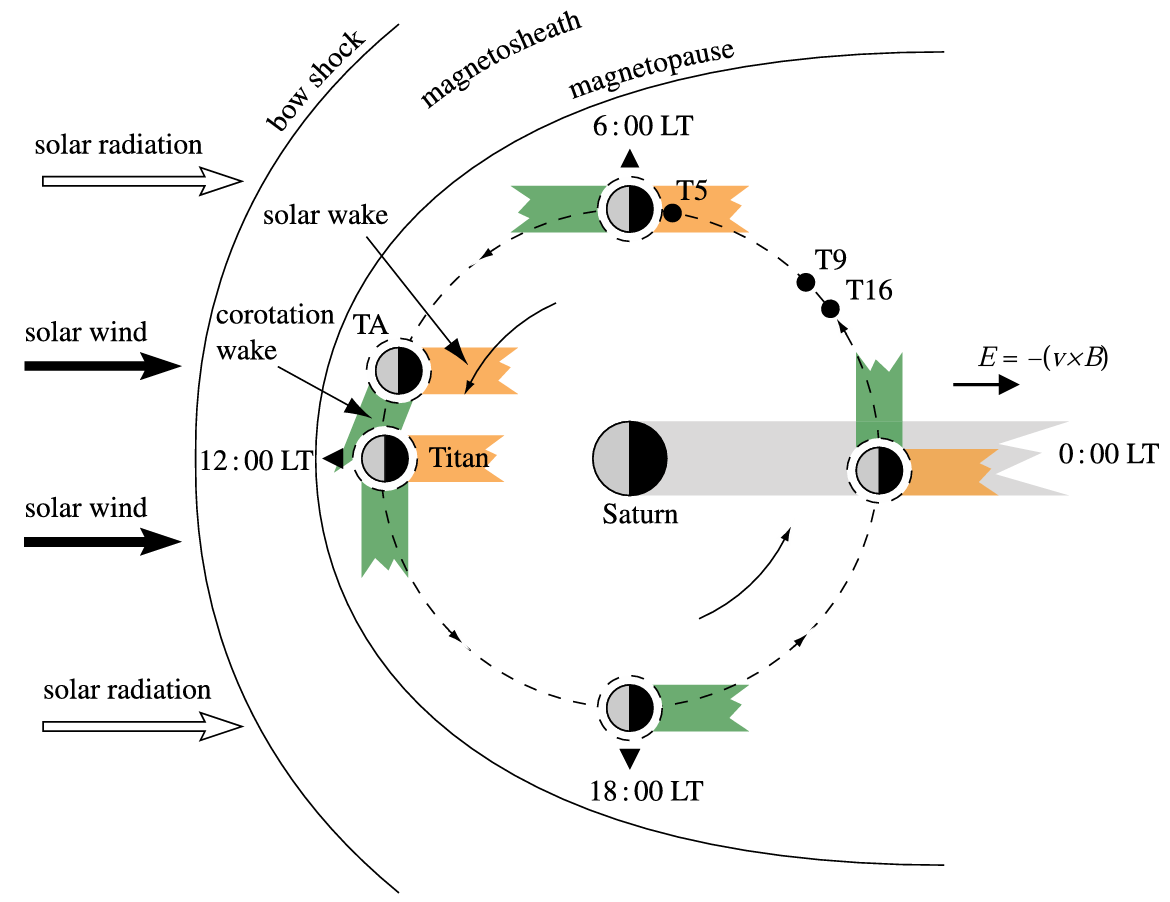
\includegraphics[width=0.7\textwidth]{wakes}
	\caption{An illustration of Titan's two plasma flow wakes in its orbit around Saturn. Taken from \textcite{ionosphere-magnetosphere-interaction-coates}.}
	\label{wakes}
\end{figure}

A planet or moon that has an ionosphere will form an induced magnetosphere if charged particles are flowing past it (section 7.2.4). This induced magnetosphere shields the body from the external magnetic field. Titan in Saturn's magnetosphere is an example of this.
% In several analyses of data recorded by instruments on the Voyager 1 when it flew by Titan in 1980 .
% Since Titan mostly resides within Saturn's magnetosphere

% The magnetic field around Titan changes rapidly only very close to its surface since it has no intrinsic magnetic field. In contrast to the planetary magnetospheres, the induced magnetosphere of Titan has no bow shock since the oncoming plasma flow is slower than both the Alfvén speed and the sound speed. Instead Alfvén wings form in front of the moon.


% Magnetotail structure

\subsection{Energetic particle interactions}

\subsubsection{Mass loading}

\subsubsection{Charge-exchange collisions}
\parencite{titan-exosphere-interaction}
Titan not having an intrinsic magnetic field makes it directly susceptible to the oncoming plasma flow, these interactions was captured using the magnetosphere imaging instrument (MIMI) and the ion and neutral mass spectrometer (INMS) onboard the Cassini spacecraft. The instruments were able to detect that energetic ions from Saturn's magnetosphere undergo charge-change collisions with slow neutral atoms in Titan's upper atmosphere, producing ENAs. The reaction describing a charge-exchange collision is \ce{X+ + Y -> X_{ENA} + Y+}, where \ce{X+} is the energetic ion, \ce{Y} is the colliding cold neutral atom, \ce{X_{ENA}} is the resulting energetic neutral atom, and \ce{Y+} is the ionized particle. Charge-exchange collisions is one of the reasons for Titan's exosphere being in thermal inequilibrium, with some other reasons being sputtering and photodissociation. Data from Cassini flybys indicated that the highest amount of particle collisions occured in the lower atmosphere causing most of the produced ENAs to be absorbed, resulting in a darker region in the ENA image of Titan's exosphere as can be seen in figure \ref{fig:ENA-image}.

\begin{figure}[htbp]
	\centering
	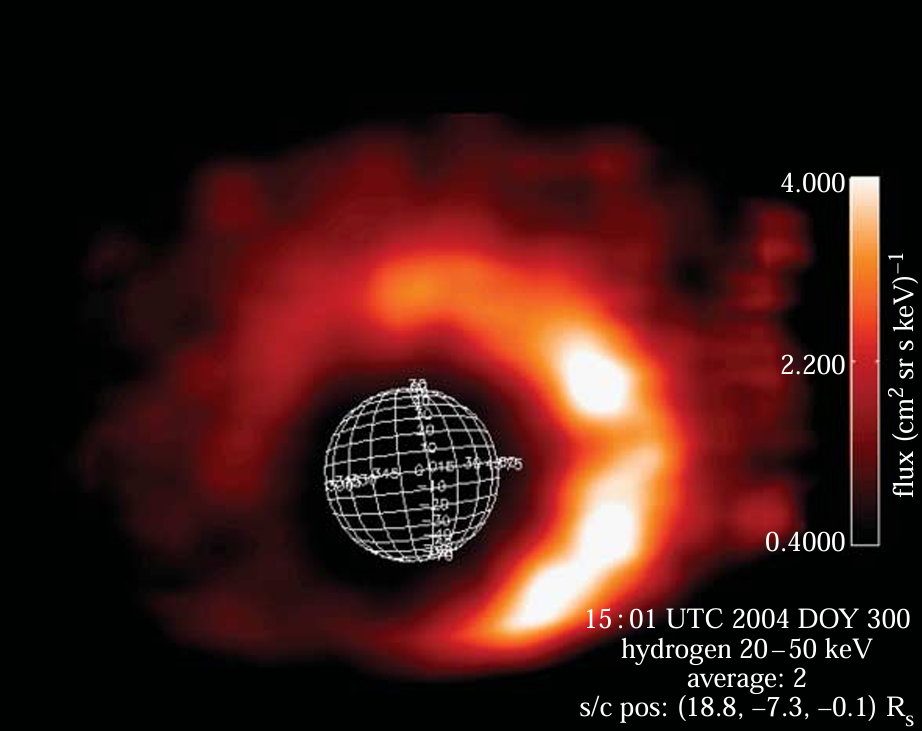
\includegraphics[width=0.7\textwidth]{ENA-image}
	\caption{Image of ENAs in Titan's exosphere taken by the MIMI during a Cassini flyby. Taken from \textcite{titan-exosphere-interaction}.}
	\label{ENA-image}
\end{figure}

% Source of plasma
 
% \subsection{}

\section{Conclusions}

\newpage
\printbibliography

\end{document}


